\documentclass[preprint,12pt]{elsarticle}
\usepackage[T1]{fontenc}
\usepackage{lmodern}
\usepackage{amsmath,amssymb}
\usepackage{booktabs}
\usepackage{graphicx}
\usepackage[hidelinks]{hyperref}
\IfFileExists{xurl.sty}{\usepackage{xurl}}{}
\setlength{\emergencystretch}{2em}
\biboptions{sort&compress}
% generated by code/make_macros.py - do not edit
\makeatletter
\expandafter\def\csname res@bdgBuildings\endcsname{1,636}
\expandafter\def\csname res@bdgSites\endcsname{19}
\expandafter\def\csname res@bestF1\endcsname{13}
\expandafter\def\csname res@bestF2\endcsname{8}
\expandafter\def\csname res@bestF3\endcsname{20}
\expandafter\def\csname res@bestF4\endcsname{55}
\expandafter\def\csname res@bestF5\endcsname{3}
\expandafter\def\csname res@filledMedPct\endcsname{0.09}
\expandafter\def\csname res@hfourP\endcsname{<0.001}
\expandafter\def\csname res@hfourShare\endcsname{95}
\expandafter\def\csname res@hfourbBeatPct\endcsname{81}
\expandafter\def\csname res@hfourbBest\endcsname{0.38}
\expandafter\def\csname res@hfourbP\endcsname{<0.001}
\expandafter\def\csname res@hfourbReactive\endcsname{0.25}
\expandafter\def\csname res@hfourbShare\endcsname{19}
\expandafter\def\csname res@holmH2\endcsname{0.310}
\expandafter\def\csname res@holmH3\endcsname{<0.001}
\expandafter\def\csname res@holmH4\endcsname{<0.001}
\expandafter\def\csname res@honeMean\endcsname{-0.012}
\expandafter\def\csname res@honeMedian\endcsname{-0.019}
\expandafter\def\csname res@honeN\endcsname{462}
\expandafter\def\csname res@honeP\endcsname{0.075}
\expandafter\def\csname res@honePos\endcsname{44}
\expandafter\def\csname res@honePsign\endcsname{0.025}
\expandafter\def\csname res@honeT\endcsname{-1.78}
\expandafter\def\csname res@honebMean\endcsname{0.057}
\expandafter\def\csname res@honebMedian\endcsname{0.057}
\expandafter\def\csname res@honebN\endcsname{462}
\expandafter\def\csname res@honebP\endcsname{<0.001}
\expandafter\def\csname res@honebPos\endcsname{63}
\expandafter\def\csname res@honebPsign\endcsname{<0.001}
\expandafter\def\csname res@honebT\endcsname{7.82}
\expandafter\def\csname res@honenofillMean\endcsname{-0.038}
\expandafter\def\csname res@honenofillMedian\endcsname{-0.050}
\expandafter\def\csname res@honenofillN\endcsname{188}
\expandafter\def\csname res@honenofillP\endcsname{<0.001}
\expandafter\def\csname res@honenofillPos\endcsname{32}
\expandafter\def\csname res@honenofillPsign\endcsname{<0.001}
\expandafter\def\csname res@honenofillT\endcsname{-3.78}
\expandafter\def\csname res@honermseMean\endcsname{0.009}
\expandafter\def\csname res@honermseMedian\endcsname{0.000}
\expandafter\def\csname res@honermseN\endcsname{462}
\expandafter\def\csname res@honermseP\endcsname{0.168}
\expandafter\def\csname res@honermsePos\endcsname{49}
\expandafter\def\csname res@honermsePsign\endcsname{1.000}
\expandafter\def\csname res@honermseT\endcsname{1.38}
\expandafter\def\csname res@hthreeN\endcsname{94}
\expandafter\def\csname res@hthreeP\endcsname{<0.001}
\expandafter\def\csname res@hthreeTauOne\endcsname{0.009}
\expandafter\def\csname res@hthreeTauTwo\endcsname{0.170}
\expandafter\def\csname res@htwoP\endcsname{0.310}
\expandafter\def\csname res@htwoRhoMae\endcsname{-0.099}
\expandafter\def\csname res@htwoRhoPeak\endcsname{-0.096}
\expandafter\def\csname res@htwoShare\endcsname{52}
\expandafter\def\csname res@keptSites\endcsname{10}
\expandafter\def\csname res@maeF1\endcsname{9.09}
\expandafter\def\csname res@maeF2\endcsname{9.21}
\expandafter\def\csname res@maeF3\endcsname{7.64}
\expandafter\def\csname res@maeF4\endcsname{7.08}
\expandafter\def\csname res@maeF5\endcsname{10.00}
\expandafter\def\csname res@maeSnoise\endcsname{7.07}
\expandafter\def\csname res@maeSscale\endcsname{7.08}
\expandafter\def\csname res@maeSshift\endcsname{7.05}
\expandafter\def\csname res@meanLoadMed\endcsname{78}
\expandafter\def\csname res@modCV\endcsname{0.16}
\expandafter\def\csname res@modLF\endcsname{-0.27}
\expandafter\def\csname res@mostAccGuard\endcsname{16}
\expandafter\def\csname res@mostAccOpen\endcsname{11}
\expandafter\def\csname res@nBM\endcsname{11,088}
\expandafter\def\csname res@nBMexcl\endcsname{772}
\expandafter\def\csname res@nBMexclPct\endcsname{7.0}
\expandafter\def\csname res@nBMused\endcsname{10,316}
\expandafter\def\csname res@nExclFlat\endcsname{207}
\expandafter\def\csname res@nExclGap\endcsname{269}
\expandafter\def\csname res@nExclMean\endcsname{45}
\expandafter\def\csname res@nExclMissing\endcsname{595}
\expandafter\def\csname res@nExclThreeH\endcsname{543}
\expandafter\def\csname res@nKept\endcsname{462}
\expandafter\def\csname res@nKeptThreeH\endcsname{188}
\expandafter\def\csname res@nMeters\endcsname{1578}
\expandafter\def\csname res@nSeasonal\endcsname{274}
\expandafter\def\csname res@negOpenFourHi\endcsname{84}
\expandafter\def\csname res@negOpenFourLo\endcsname{82}
\expandafter\def\csname res@negOpenHi\endcsname{84}
\expandafter\def\csname res@negOpenLo\endcsname{65}
\expandafter\def\csname res@negT1F1\endcsname{84}
\expandafter\def\csname res@negT1F2\endcsname{82}
\expandafter\def\csname res@negT1F3\endcsname{83}
\expandafter\def\csname res@negT1F4\endcsname{82}
\expandafter\def\csname res@negT1F5\endcsname{65}
\expandafter\def\csname res@negT1GF1\endcsname{0}
\expandafter\def\csname res@negT1GF2\endcsname{0}
\expandafter\def\csname res@negT1GF3\endcsname{0}
\expandafter\def\csname res@negT1GF4\endcsname{0}
\expandafter\def\csname res@negT1GF5\endcsname{0}
\expandafter\def\csname res@negT1GSnoise\endcsname{0}
\expandafter\def\csname res@negT1GSscale\endcsname{0}
\expandafter\def\csname res@negT1GSshift\endcsname{0}
\expandafter\def\csname res@negT1Snoise\endcsname{67}
\expandafter\def\csname res@negT1Sscale\endcsname{0}
\expandafter\def\csname res@negT1Sshift\endcsname{97}
\expandafter\def\csname res@negT1reactive\endcsname{2}
\expandafter\def\csname res@negT2F1\endcsname{0}
\expandafter\def\csname res@negT2F2\endcsname{0}
\expandafter\def\csname res@negT2F3\endcsname{0}
\expandafter\def\csname res@negT2F4\endcsname{0}
\expandafter\def\csname res@negT2F5\endcsname{0}
\expandafter\def\csname res@negT2GF1\endcsname{0}
\expandafter\def\csname res@negT2GF2\endcsname{0}
\expandafter\def\csname res@negT2GF3\endcsname{0}
\expandafter\def\csname res@negT2GF4\endcsname{0}
\expandafter\def\csname res@negT2GF5\endcsname{0}
\expandafter\def\csname res@negT2GSnoise\endcsname{0}
\expandafter\def\csname res@negT2GSscale\endcsname{0}
\expandafter\def\csname res@negT2GSshift\endcsname{0}
\expandafter\def\csname res@negT2Snoise\endcsname{0}
\expandafter\def\csname res@negT2Sscale\endcsname{0}
\expandafter\def\csname res@negT2Sshift\endcsname{0}
\expandafter\def\csname res@negT2reactive\endcsname{1}
\expandafter\def\csname res@rankF1\endcsname{3.39}
\expandafter\def\csname res@rankF2\endcsname{3.64}
\expandafter\def\csname res@rankF3\endcsname{2.25}
\expandafter\def\csname res@rankF4\endcsname{1.73}
\expandafter\def\csname res@rankF5\endcsname{3.99}
\expandafter\def\csname res@relbiasF1\endcsname{-0.0}
\expandafter\def\csname res@relbiasF2\endcsname{-0.0}
\expandafter\def\csname res@relbiasF3\endcsname{+0.3}
\expandafter\def\csname res@relbiasF4\endcsname{+0.3}
\expandafter\def\csname res@relbiasF5\endcsname{+10.9}
\expandafter\def\csname res@relmaeF1\endcsname{13.1}
\expandafter\def\csname res@relmaeF2\endcsname{14.2}
\expandafter\def\csname res@relmaeF3\endcsname{11.1}
\expandafter\def\csname res@relmaeF4\endcsname{10.2}
\expandafter\def\csname res@relmaeF5\endcsname{14.1}
\expandafter\def\csname res@relmaeSnoise\endcsname{10.2}
\expandafter\def\csname res@relmaeSscale\endcsname{10.2}
\expandafter\def\csname res@relmaeSshift\endcsname{10.2}
\expandafter\def\csname res@rhoBiasGuard\endcsname{0.16}
\expandafter\def\csname res@rhoBiasOpen\endcsname{0.17}
\expandafter\def\csname res@rhoMaeGuard\endcsname{-0.00}
\expandafter\def\csname res@rhoMaeOpen\endcsname{-0.29}
\expandafter\def\csname res@robMaxAbsTau\endcsname{0.06}
\expandafter\def\csname res@robb05Excl\endcsname{4394}
\expandafter\def\csname res@robb05Mean\endcsname{+0.028}
\expandafter\def\csname res@robb05P\endcsname{<0.001}
\expandafter\def\csname res@robb05Pos\endcsname{55}
\expandafter\def\csname res@robb20Excl\endcsname{4}
\expandafter\def\csname res@robb20Mean\endcsname{-0.037}
\expandafter\def\csname res@robb20P\endcsname{<0.001}
\expandafter\def\csname res@robb20Pos\endcsname{39}
\expandafter\def\csname res@robdc10Excl\endcsname{778}
\expandafter\def\csname res@robdc10Mean\endcsname{-0.006}
\expandafter\def\csname res@robdc10P\endcsname{0.393}
\expandafter\def\csname res@robdc10Pos\endcsname{47}
\expandafter\def\csname res@robdc30Excl\endcsname{771}
\expandafter\def\csname res@robdc30Mean\endcsname{-0.014}
\expandafter\def\csname res@robdc30P\endcsname{0.041}
\expandafter\def\csname res@robdc30Pos\endcsname{44}
\expandafter\def\csname res@scaleHi\endcsname{14.3}
\expandafter\def\csname res@scaleLo\endcsname{6.3}
\expandafter\def\csname res@scaleMed\endcsname{9.7}
\expandafter\def\csname res@shGuardHi\endcsname{0.37}
\expandafter\def\csname res@shGuardLo\endcsname{0.32}
\expandafter\def\csname res@shOpenHi\endcsname{-0.10}
\expandafter\def\csname res@shOpenLo\endcsname{-0.33}
\expandafter\def\csname res@shT1F1\endcsname{-0.33}
\expandafter\def\csname res@shT1F2\endcsname{-0.31}
\expandafter\def\csname res@shT1F3\endcsname{-0.28}
\expandafter\def\csname res@shT1F4\endcsname{-0.28}
\expandafter\def\csname res@shT1F5\endcsname{-0.10}
\expandafter\def\csname res@shT1GF1\endcsname{0.32}
\expandafter\def\csname res@shT1GF2\endcsname{0.32}
\expandafter\def\csname res@shT1GF3\endcsname{0.32}
\expandafter\def\csname res@shT1GF4\endcsname{0.33}
\expandafter\def\csname res@shT1GF5\endcsname{0.37}
\expandafter\def\csname res@shT1GSnoise\endcsname{0.40}
\expandafter\def\csname res@shT1GSscale\endcsname{0.55}
\expandafter\def\csname res@shT1GSshift\endcsname{0.39}
\expandafter\def\csname res@shT1Snoise\endcsname{-0.13}
\expandafter\def\csname res@shT1Sscale\endcsname{0.89}
\expandafter\def\csname res@shT1Sshift\endcsname{-0.47}
\expandafter\def\csname res@shT1reactive\endcsname{0.25}
\expandafter\def\csname res@shT2F1\endcsname{1.00}
\expandafter\def\csname res@shT2F2\endcsname{1.00}
\expandafter\def\csname res@shT2F3\endcsname{1.00}
\expandafter\def\csname res@shT2F4\endcsname{1.00}
\expandafter\def\csname res@shT2F5\endcsname{1.00}
\expandafter\def\csname res@shT2GF1\endcsname{1.00}
\expandafter\def\csname res@shT2GF2\endcsname{1.00}
\expandafter\def\csname res@shT2GF3\endcsname{1.00}
\expandafter\def\csname res@shT2GF4\endcsname{1.00}
\expandafter\def\csname res@shT2GF5\endcsname{1.00}
\expandafter\def\csname res@shT2GSnoise\endcsname{1.00}
\expandafter\def\csname res@shT2GSscale\endcsname{1.00}
\expandafter\def\csname res@shT2GSshift\endcsname{1.00}
\expandafter\def\csname res@shT2Snoise\endcsname{1.00}
\expandafter\def\csname res@shT2Sscale\endcsname{1.00}
\expandafter\def\csname res@shT2Sshift\endcsname{1.00}
\expandafter\def\csname res@shT2reactive\endcsname{0.13}
\expandafter\def\csname res@synFriedP\endcsname{<0.001}
\expandafter\def\csname res@synFriedPg\endcsname{<0.001}
\expandafter\def\csname res@useE\endcsname{175}
\expandafter\def\csname res@useEpa\endcsname{45}
\expandafter\def\csname res@useO\endcsname{92}
\expandafter\def\csname res@usePs\endcsname{74}
\expandafter\def\csname res@worstF1\endcsname{27}
\expandafter\def\csname res@worstF2\endcsname{33}
\expandafter\def\csname res@worstF3\endcsname{1}
\expandafter\def\csname res@worstF4\endcsname{1}
\expandafter\def\csname res@worstF5\endcsname{37}
\makeatother
\newcommand{\res}[1]{\ifcsname res@#1\endcsname\csname res@#1\endcsname\else\textbf{??#1??}\fi}

\ifdefined\ANON
\newcommand{\repolink}{a repository whose address is given on the title page (withheld for anonymized review)}
\else
\newcommand{\repolink}{\url{https://github.com/Thanh-Van-2001/battery-forecast-value}}
\fi

\journal{Energy and Buildings}

\begin{document}

\begin{frontmatter}

\title{The most accurate load forecast is not the most valuable: a pre-specified study of battery peak shaving under demand charges in \res{nKept} buildings}

% main_anon.tex defines \ANON and inputs this file: the anonymized review copy.
\ifdefined\ANON\else
\author[tsg]{Thanh Van Nguyen\corref{cor1}}
\ead{felicenguyen2001@gmail.com}
\cortext[cor1]{Corresponding author.}
\affiliation[tsg]{organization={Tsinghua Shenzhen International Graduate School, Tsinghua University},
            city={Shenzhen},
            country={China}}
\fi

\begin{abstract}
Load forecasts for battery scheduling are usually chosen by accuracy metrics such as the mean absolute error. We ask whether the most accurate forecast also saves the most money. In a pre-registered study of \res{nKept} non-residential buildings from the Building Data Genome 2 data set, a behind-the-meter battery was scheduled day-ahead from five standard forecasters under a time-of-use tariff with and without a monthly demand charge, and every schedule was costed on the buildings' actual 2017 load. Under the demand charge, the ranking of forecasters by accuracy did not agree with their ranking by saving (mean Kendall $\tau=\res{honeMean}$ with open-loop execution and $\res{honebMean}$ with a real-time peak guard), and the most accurate forecaster was the most valuable in only \res{mostAccOpen}--\res{mostAccGuard}\% of building-months, below the 20\% expected by chance. The least accurate model on average, a 0.9-quantile forecaster, saved the most. At equal error, a one-hour timing error destroyed the saving while a uniform over-forecast of about 10\% kept most of it. How the schedule was executed mattered more than the forecaster: executed open loop, the schedules of the four point forecasters raised the bill above the no-battery bill in \res{negOpenFourLo}--\res{negOpenFourHi}\% of buildings (\res{negT1F5}\% for the quantile forecaster), while a simple guard turned all of them into savings and beat a forecast-free reactive rule in \res{hfourbBeatPct}\% of buildings. Without a demand charge, all forecasters captured the full saving. Forecasts for storage under demand charges should be judged by the bill they produce, not by accuracy.

\end{abstract}

\begin{keyword}
Load forecasting \sep Battery energy storage \sep Demand charge \sep Peak shaving \sep Forecast value \sep Quantile forecasting \sep Non-residential buildings
\end{keyword}

\end{frontmatter}

\section{Introduction}\label{sec:intro}

Commercial and institutional buildings in many markets pay a demand charge on their highest metered power in a billing month in addition to an energy charge per kilowatt-hour. A behind-the-meter battery can lower that charge by discharging during the peak, and it can also shift energy from expensive to cheap hours~\cite{oudalov2007sizing,leadbetter2012battery,hanna2014dispatch,papadopoulos2020peak}. Both uses need a forecast of the building's load, and the forecast is usually chosen the way forecasts are chosen everywhere: by its mean absolute error (MAE), its root mean squared error or a percentage error on held-out data~\cite{hong2016probabilistic,wang2019smartmeter,hyndman2006another}. Large benchmarks of building load forecasting rank models in exactly this way~\cite{emami2023buildingsbench,miller2020gepiii}.

There are reasons to doubt that accuracy ranks forecasts by what they are worth to a battery. A demand charge depends on a single hour per month, and an error that makes the forecast too low at a charging hour can set a new peak, while an error of the same size in the other direction only keeps charge in reserve. That the value of a forecast depends on the user's loss, not only on its error, is an old idea in forecast verification~\cite{murphy1993good}; a point forecast is optimal only relative to a scoring function~\cite{gneiting2011point,gneiting2007scoring}, and the value of probabilistic forecasts for decisions under asymmetric penalties is well documented in energy trading~\cite{pinson2007trading}. Decision-focused learning trains forecasters on the cost of the decision they feed instead of on their error~\cite{donti2017task,elmachtoub2022spo,mandi2024dfl,sadana2025survey}, and recent work applies the idea to demand-charge storage~\cite{kim2025neural} and to photovoltaic-battery scheduling in twenty buildings~\cite{depoortere2026dfl}. What is missing is a measurement, on many buildings, of how far the usual accuracy metric is from the decision value of the forecasts that practitioners actually use, of which properties of the error drive the gap, and of whether a simple asymmetric score closes it.

This paper provides that measurement. We schedule a battery day-ahead in each of \res{nKept} buildings of the Building Data Genome 2 data set~\cite{miller2020bdg2} from five standard forecasters, execute every schedule against the actual 2017 load, and compare the share of the perfect-information saving each forecaster captures with its accuracy. The analysis plan, with its primary hypothesis and test, was committed to the study's version-controlled repository before the data were downloaded; three amendments, the last made after the results and an independent review and including a bug fix, are disclosed, and the registered test is reported on the registered simulation. Synthetic forecasts with exactly the MAE of the best model but a single type of error each (uniform over- and under-forecasts, independent and correlated noise, a late ramp) separate which errors matter. Each schedule is executed in two ways, open loop and with a real-time guard that stops the battery from charging into the month's peak, which separates the value of the forecast from that of the controller.

Under the demand charge, the pre-specified test found no agreement between the ranking of forecasters by MAE and their ranking by saving: the mean Kendall rank correlation across buildings was \res{voneMean} (95\% CI \res{voneLo} to \res{voneHi}). The sign of the error explains the gap. The 0.9-quantile forecaster, the least accurate on average, captured the largest saving; at equal MAE a uniform over-forecast kept \res{shT1Sscale} of the attainable saving while a uniform under-forecast lost money when executed open loop; and ranking by the 0.9 pinball loss agreed with value ($\tau=\res{pinOpenMean}$), as did MAE among the four unbiased forecasters ($\tau=\res{fourOpenMean}$). The controller mattered more than the forecaster: open-loop schedules raised the bill in \res{negOpenFourLo}--\res{negOpenFourHi}\% of buildings, whereas the guarded schedules saved money and beat a forecast-free rule in \res{beatReactLo}--\res{beatReactHi}\% of buildings. The saving at stake is small, \res{pctT1PI}\% of the median bill with perfect information, which is why errors of a few per cent in the wrong direction can erase it. Without a demand charge every forecaster captured the full saving. Section~\ref{sec:related} reviews related work, Section~\ref{sec:model} the data and decision model, Section~\ref{sec:design} the forecasters and pre-specified design, Section~\ref{sec:results} the results, and Section~\ref{sec:discussion} their implications and limits.

\section{Related work}\label{sec:related}

\paragraph{Batteries for demand-charge management} Sizing and operating storage for peak shaving is a well-studied problem~\cite{oudalov2007sizing,leadbetter2012battery,papadopoulos2020peak}. Schedules are typically computed from a load (and, with photovoltaics, a generation) forecast by linear or mixed-integer programming, so that forecast errors reduce the realised saving~\cite{hanna2014dispatch}. Recent studies optimise storage and vehicle-to-building resources for commercial buildings, in one case with machine-learned load forecasts~\cite{ghafoori2023v2b,jiang2026v2b}, and handle forecast error with robust model predictive control~\cite{mary2025rmpc}. These studies optimise a controller for one forecaster or a few buildings; they do not ask how the choice among forecasters, judged by accuracy, relates to the bill across a population of buildings.

\paragraph{Evaluating load forecasts} Building and smart-meter load forecasting is evaluated almost entirely by error metrics~\cite{hong2016probabilistic,wang2019smartmeter}, including in the largest recent benchmark~\cite{emami2023buildingsbench}. Soman et al.~\cite{soman2020peak} distinguish predicting which hours will be the peak from predicting the whole load curve, and argue that the former is what battery-based optimisation on a campus microgrid needs. Gneiting~\cite{gneiting2011point} shows more generally that a point forecast is optimal only relative to a scoring function, so that ranking forecasts by MAE implicitly assumes that the decision maker's loss is symmetric and linear in the error.

\paragraph{Decision-focused and value-oriented forecasting} Decision-focused learning trains a predictor on the cost of the downstream optimisation instead of on its error~\cite{elmachtoub2022spo,mandi2024dfl,sadana2025survey}. In energy, value-oriented forecasting has been applied to trading renewable output~\cite{stratigakos2021value}, to demand-charge storage with a jointly trained forecaster and controller~\cite{kim2025neural}, and to residential photovoltaic-battery scheduling on twenty buildings, where it lowered costs by a few per cent at a loss of accuracy~\cite{depoortere2026dfl}. The present study is complementary. It proposes no new training method; it measures how well the accuracy of conventional forecasters predicts their decision value on \res{nKept} buildings and decomposes the gap by type of error and by controller, which indicates when decision-focused training, or simply a different choice among existing forecasters, is worth the effort.

\section{Data and decision model}\label{sec:model}

\subsection{Buildings}
The Building Data Genome 2 data set contains hourly meter readings from \res{bdgBuildings} non-residential buildings at \res{bdgSites} sites in North America and Europe for 2016 and 2017~\cite{miller2020bdg2}. We use its cleaned electricity meters (\res{nMeters} meters), 2016 for fitting and 2017 for testing. A meter is excluded if more than 5\% of its hours are missing in either year (\res{nExclMissing} meters), if it repeats the same reading for 72 hours or more, a sign of a stuck meter (\res{nExclFlat}), if a gap exceeds 24 hours (\res{nExclGap}), or if its mean load is below 10 kWh per hour (\res{nExclMean}). Gaps of up to three hours are interpolated linearly; longer gaps, in \res{nSeasonal} of the \res{nKept} remaining buildings, are filled with the load at the same hour one week earlier. The median building has \res{filledMedPct}\% of its hours filled. The \res{nKept} buildings come from \res{keptSites} sites; the most common uses are education (\res{useE}), office (\res{useO}) and public services (\res{usePs}), and the median building draws \res{meanLoadMed} kW on average. Each building is matched to its site's air temperature.

\subsection{Tariffs and battery}
Two tariffs are used. Both charge 0.20~\$/kWh between 12:00 and 18:00 on weekdays and 0.10~\$/kWh otherwise. Tariff T1 adds a demand charge of $\lambda=20$~\$/kW on the highest hourly grid draw of each calendar month; tariff T2 has no demand charge. The battery's power rating $P$ is 10\% of the building's 2016 peak load and its capacity $E=2P$ (two hours). Round-trip efficiency is 90\%, split equally between charging and discharging ($\eta=\sqrt{0.9}$), the state of charge is kept between 10\% and 90\% of $E$, and the battery does not export to the grid.

\subsection{Day-ahead schedule}
At midnight before day $d$, the operator chooses charging and discharging powers $c_t,\delta_t$ for the 24 hours $t$ of the day from a forecast $\hat L_t$ of the load by the linear program
\begin{align}
\min_{c,\delta,s,g,z}\ & \sum_{t=1}^{24} p_t g_t + \lambda z \label{eq:lp}\\
\text{s.t.}\ & s_{t+1}=s_t+\eta c_t-\delta_t/\eta,\quad g_t=\hat L_t+c_t-\delta_t,\quad g_t\ge 0,\quad z\ge g_t, \nonumber\\
& z\ge \bar G_{m(d)},\quad 0\le c_t,\delta_t\le P,\quad 0.1E\le s_t\le 0.9E,\quad s_1=s_{25}=0.5E, \nonumber
\end{align}
where $p_t$ is the energy price, $g_t$ the grid draw and $\bar G_{m(d)}$ the highest realised grid draw so far in the month of day $d$. The term $\lambda z$ thus charges only for raising the month's peak, and under T2 ($\lambda=0$) the program is pure energy arbitrage. The program is solved with HiGHS for every building, day and forecaster.

\subsection{Execution and benchmarks}
The schedule is executed against the actual load $L_t$ in one of two ways.
\begin{itemize}
\item \emph{Open loop}: the scheduled powers are applied as planned, clipped only to keep the state of charge within its limits and to avoid export.
\item \emph{Guarded} (Amendment~2, Section~\ref{sec:design}): the scheduled powers are applied, but charging is reduced so that the realised grid draw never exceeds the month-to-date realised peak, and when the actual load alone exceeds that peak the battery discharges, as far as its power and charge allow, to hold the grid draw at the peak. Under T2 the guard has nothing to do and the two executions coincide.
\end{itemize}
Three benchmarks complete the comparison: no battery; \emph{perfect information}, the same daily program solved with the actual load; and a \emph{reactive rule} that needs no forecast, which under T1 discharges whenever the load exceeds the month-to-date peak and otherwise charges in cheap hours without creating a new peak, and under T2 charges in cheap hours and discharges in expensive ones. Each day's schedule starts and ends at half charge; energy left above that level by open-loop clipping is forfeited, which penalises poor forecasts equally for all forecasters.

\subsection{Decision value}
The monthly bill of each policy is the energy cost of its grid draw plus, under T1, $\lambda$ times the month's highest hourly grid draw. The decision value of a forecaster in a building-month is the share of the perfect-information saving that it captures,
\begin{equation}
\text{share}=\frac{\text{bill(no battery)}-\text{bill(forecaster)}}{\text{bill(no battery)}-\text{bill(perfect information)}},
\end{equation}
which is 1 for a forecaster as good as perfect information, 0 for one that saves nothing and negative for one that raises the bill. Building-months in which perfect information saves less than 0.5\% of the no-battery bill are excluded from share-based analyses because the share is unstable there (\res{nBMexcl} of \res{nBM} building-month-tariff cells, \res{nBMexclPct}\%). Annual shares sum the bills over the remaining months.

\section{Forecasters and pre-registered design}\label{sec:design}

\subsection{Forecasters}
All forecasters predict the 24 hourly loads of day $d$ at midnight, using loads up to the previous day and the day's temperature. F1 repeats the load of the same hour one day earlier and F2 the load of the same hour one week earlier. F3 is a ridge regression and F4 a gradient-boosted tree model (LightGBM~\cite{ke2017lightgbm}, 400 trees) on hour-of-day and day-of-week indicators, the loads 24, 48 and 168 hours earlier, the temperature, its square and heating and cooling degree terms. F5 is the same LightGBM model trained on the pinball loss of the 0.9 quantile, a peak-conservative forecaster. Models are fitted per building on 2016 and are not refitted. The temperature is the observed value, which amounts to a perfect weather forecast for all forecasters.

To separate the type of error from its size, three synthetic forecasts are built from the actual load with the same MAE as F4 in every building-month: actual load plus Gaussian noise (\emph{noise}); the actual load moved towards the load one hour earlier by a multiple of their difference, so that rises and peaks are predicted late (\emph{1-h shift}); and the actual load scaled up by a constant factor within the month (\emph{uniform over-forecast}). Matching the MAE makes that factor equal to F4's relative MAE in the month, \res{scaleMed}\% at the median (interquartile range \res{scaleLo}--\res{scaleHi}\%); the analysis plan had described this error as a 5\% scale error, but the matched-MAE construction it specified fixes the size.

Accuracy is measured per building-month by the MAE, the RMSE, the mean absolute percentage error, the absolute error at the hour of the actual daily peak, the error of the forecast daily peak magnitude and the timing error of the forecast daily peak. Over the test year the median MAE was \res{maeF4} kWh per hour for F4, \res{maeF3} for F3, \res{maeF1} for F1, \res{maeF2} for F2 and \res{maeF5} for F5 (relative to the mean load: \res{relmaeF4}\%, \res{relmaeF3}\%, \res{relmaeF1}\%, \res{relmaeF2}\% and \res{relmaeF5}\%). Within a building-month the two summaries rank the forecasters identically; ranked by MAE across building-months, F4 was most accurate on average (mean rank \res{rankF4}, best in \res{bestF4}\%) and F5 least (mean rank \res{rankF5}, last in \res{worstF5}\%). The median relative bias was close to zero for F1--F4 and \res{relbiasF5}\% for F5.

\subsection{Pre-registration and amendments}
The questions, hypotheses, primary test, forecasters, tariffs, battery and robustness checks were fixed in an analysis plan committed to the study repository (\url{\repoURL}, file \texttt{PLAN.md}) before any data were downloaded. Two amendments followed, both before the full run and both in the repository. The first, written with the code and before any data were loaded, fixed the exclusion rule for building-months with a negligible perfect-information saving and the reset of the state of charge. The second followed a pipeline check on six buildings whose outcomes were seen: the original rule of excluding any building with a gap longer than three hours kept only \res{nKeptThreeH} of the \res{nMeters} meters (\res{nExclThreeH} excluded for that reason alone), so longer gaps were filled as described above; and because every forecaster executed open loop raised the bill in those six buildings, the guarded execution was added as a secondary controller. The hypotheses and their tests were not changed, and the primary results below are those of the registered open-loop controller.

\subsection{Hypotheses and tests}
\begin{itemize}
\item[H1] (primary) Under T1, the ranking of F1--F5 by MAE agrees with their ranking by captured share. For each building-month we compute Kendall's $\tau$ between the negative MAE and the share across the five forecasters, average it over the months of each building, and test the mean over buildings against zero with a $t$-test and a sign test.
\item[H2] Under T1, the error of the forecast daily peak predicts the share better than the MAE (per-building Spearman correlations over forecaster-months, compared by a Wilcoxon signed-rank test).
\item[H3] Agreement between accuracy and value is higher under T2 than under T1 (paired Wilcoxon test over buildings).
\item[H4] Under T1 the reactive rule captures at least as large an annual share as the best forecaster in at least half of the buildings (sign test).
\end{itemize}
H2--H4 are adjusted with Holm's method. Secondary analyses (labelled as such) repeat H1 and H4 for the guarded controller (H1b, H4b) and compare the synthetic error types with Friedman tests. Robustness checks, all listed in the plan, use battery powers of 5\% and 20\% of the peak, demand charges of 10 and 30~\$/kW, RMSE in place of MAE, and the buildings without filled gaps.

\section{Results}\label{sec:results}

The analyses use \res{nBMused} building-month-tariff cells after the exclusion rule of Section~\ref{sec:model}. Unless stated otherwise, results refer to tariff T1, the demand-charge tariff.

\subsection{Accuracy does not rank forecasters by value (H1)}

Executed open loop, the ranking of the five forecasters by MAE did not agree with their ranking by captured share. The mean over buildings of the per-building Kendall $\tau$ was $\res{honeMean}$ (median $\res{honeMedian}$; positive in \res{honePos}\% of buildings; $t=\res{honeT}$, $p=\res{honeP}$; sign test $p=\res{honePsign}$), so the primary hypothesis is not supported; if anything, the more accurate forecaster tended to capture slightly less. Ranking by RMSE instead gave $\tau=\res{honermseMean}$ ($p=\res{honermseP}$), and the \res{honenofillN} buildings without filled gaps gave $\tau=\res{honenofillMean}$ ($p=\res{honenofillP}$). With the guarded controller (H1b, secondary) the agreement was positive but weak: $\tau=\res{honebMean}$, positive in \res{honebPos}\% of buildings ($p=\res{honebP}$).

An exploratory count makes the size of the gap concrete. In a building-month, the forecaster with the lowest MAE was also the one with the largest captured share in \res{mostAccOpen}\% of cases with open-loop execution and \res{mostAccGuard}\% with the guard. If accuracy and value were unrelated the figure would be 20\%; it is lower because the least accurate forecaster was usually the most valuable (Section~\ref{sec:res-errors}).

\subsection{The controller matters more than the forecaster (H4)}

\begin{figure}[t]
\centering
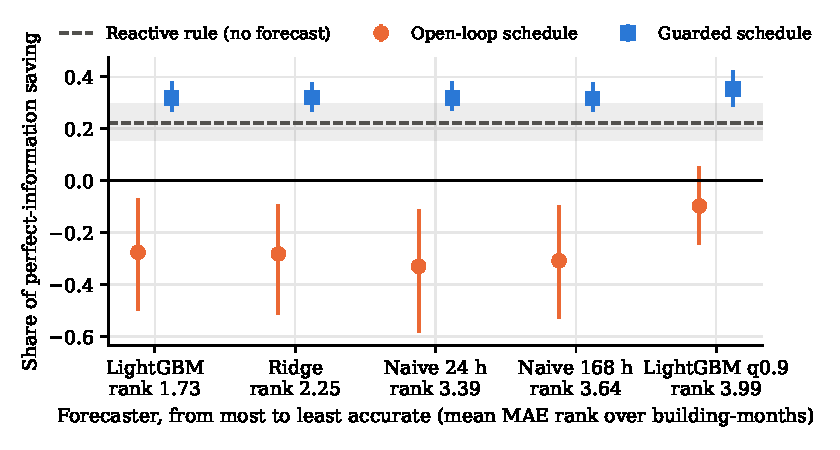
\includegraphics[width=\linewidth]{figures/fig_share_by_forecaster.pdf}
\caption{Annual share of the perfect-information saving under the demand-charge tariff, by forecaster (ordered by mean MAE rank, 1 = most accurate) and controller. Points are medians over \res{nKept} buildings, bars interquartile ranges; the dashed line and band are the median and interquartile range of the forecast-free reactive rule. Negative values mean a higher bill than without a battery.}\label{fig:share}
\end{figure}

Figure~\ref{fig:share} shows the annual captured share by forecaster and controller. Executed open loop, every forecaster had a negative median share, from $\res{shOpenLo}$ to $\res{shOpenHi}$: the battery raised the bill above the no-battery bill in \res{negT1F1}\% (F1), \res{negT1F2}\% (F2), \res{negT1F3}\% (F3), \res{negT1F4}\% (F4) and \res{negT1F5}\% (F5) of buildings. The mechanism is the asymmetry of the demand charge. The schedule charges in the cheap hours before noon to discharge in the expensive afternoon; when the actual load in a charging hour turns out higher than forecast, the charging power is added to it and can set a new monthly peak. A full-power charge at the hour that becomes the month's peak costs $\lambda P$, as much as a perfectly timed full discharge saves, and the energy arbitrage earns far less than that. The reactive rule, which never charges above the month-to-date peak, captured a median share of $\res{shT1reactive}$ and was at least as good as the best open-loop forecaster in \res{hfourShare}\% of buildings (H4, Holm-adjusted $p=\res{holmH4}$).

The guard removes the asymmetry. With guarded execution, no forecaster raised the annual bill in any building, and the median shares ranged from $\res{shGuardLo}$ to $\res{shGuardHi}$, and the best forecaster of each building beat the reactive rule in \res{hfourbBeatPct}\% of buildings (medians $\res{hfourbBest}$ against $\res{hfourbReactive}$; H4b, $p=\res{hfourbP}$). The reactive rule is a lower bound for a well-tuned forecast-free rule: it charges whenever energy is cheap, including on weekends when no expensive hours follow, and because every day starts at half charge it pays for energy that it never uses. Even so, the step from open loop to the guard changed the median share by more than any choice among the five forecasters did under either controller.

\subsection{Which errors matter (H2)}\label{sec:res-errors}

\begin{figure}[t]
\centering
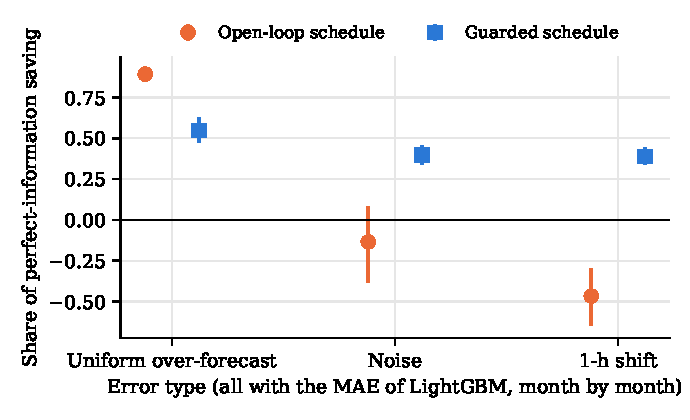
\includegraphics[width=0.78\linewidth]{figures/fig_synthetic.pdf}
\caption{Annual share of the perfect-information saving for three synthetic forecasts with the same MAE as LightGBM in every building-month (medians and interquartile ranges over buildings, demand-charge tariff).}\label{fig:syn}
\end{figure}

The synthetic forecasts isolate the type of error (Figure~\ref{fig:syn}). At the same MAE as F4, a uniform over-forecast kept a median share of $\res{shT1Sscale}$ with open-loop execution, random noise gave $\res{shT1Snoise}$ and a one-hour delay $\res{shT1Sshift}$ (Friedman $p\res{synFriedP}$). With the guard the three were $\res{shT1GSscale}$, $\res{shT1GSnoise}$ and $\res{shT1GSshift}$ (Friedman $p\res{synFriedPg}$): the guard rescues the noisy and late forecasts, and the over-forecast remains the most valuable. Errors that make the forecast load too low at the hours the battery charges are the expensive ones; errors that make it too high are cheap, because they lead the schedule to keep charge in reserve.

\begin{figure}[t]
\centering
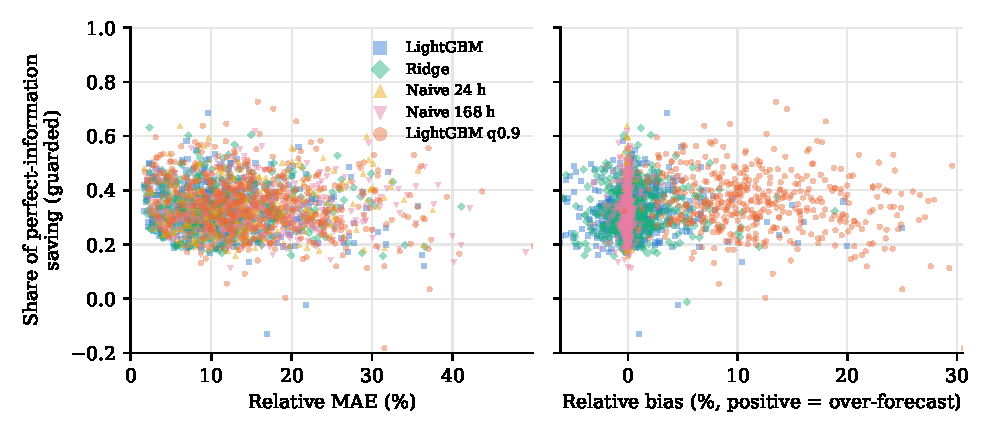
\includegraphics[width=\linewidth]{figures/fig_accuracy_vs_value.pdf}
\caption{Accuracy and bias against value. Each point is a building and forecaster: relative MAE (left) and relative bias (right) over the test year against the annual share of the perfect-information saving with guarded execution (demand-charge tariff).}\label{fig:acc}
\end{figure}

The real forecasters show the same pattern (Figure~\ref{fig:acc}). The 0.9-quantile model F5 was the least accurate on average (mean MAE rank \res{rankF5} of 5 across building-months, last in \res{worstF5}\%, against \res{rankF4} for F4) and the only one with a material bias (\res{relbiasF5}\%), and it captured the largest median share under both controllers (open loop $\res{shT1F5}$, guarded $\res{shT1GF5}$). Across buildings and forecasters, the Spearman correlation of the annual share with accuracy (negative relative MAE) was $\res{rhoMaeOpen}$ for open-loop schedules and $\res{rhoMaeGuard}$ with the guard, and with relative bias $\res{rhoBiasOpen}$ and $\res{rhoBiasGuard}$ (exploratory). The pre-registered H2 asked whether the error of the forecast daily peak predicts value better than the MAE; it did not (mean per-building Spearman correlations $\res{htwoRhoPeak}$ and $\res{htwoRhoMae}$, Holm-adjusted $p=\res{holmH2}$). Both are negative under open loop: the peak magnitude, like the average, is the wrong target when the cost of an error depends on its sign.

\subsection{Without a demand charge, accuracy does not matter (H3)}

Under the time-of-use tariff T2 every forecaster captured the full perfect-information saving: the median annual share was $\res{shT2F1}$ for each of F1--F5 and no building-forecaster pair was below zero. The schedule of a pure arbitrage program depends on the prices, not on the load, as long as the load exceeds the battery's discharge. Kendall's $\tau$ is therefore undefined in most buildings; in the \res{hthreeN} buildings where the shares differed under both tariffs, agreement was higher under T2 than under T1 ($\res{hthreeTauTwo}$ against $\res{hthreeTauOne}$; H3, Holm-adjusted $p=\res{holmH3}$), but the differences it ranks are negligible.

\subsection{Robustness}

\begin{table}[t]
\centering
\footnotesize
\caption{Primary test (H1) under alternative batteries and demand charges: mean per-building Kendall $\tau$ between accuracy (negative MAE) and captured share, open-loop execution unless stated, demand-charge tariff. Excluded: building-month-tariff cells removed by the 0.5\% rule.}\label{tab:rob}
\setlength{\tabcolsep}{4pt}
\begin{tabular}{lrrrr}
\toprule
Setting & Mean $\tau$ & $p$ & $\tau>0$ (\%) & Excluded \\
\midrule
Base: $P$ = 10\% of peak, 20 \$/kW & $\res{honeMean}$ & \res{honeP} & \res{honePos} & \res{nBMexcl} \\
$P$ = 5\% of peak & $\res{robb05Mean}$ & \res{robb05P} & \res{robb05Pos} & \res{robb05Excl} \\
$P$ = 20\% of peak & $\res{robb20Mean}$ & \res{robb20P} & \res{robb20Pos} & \res{robb20Excl} \\
Demand charge 10 \$/kW & $\res{robdc10Mean}$ & \res{robdc10P} & \res{robdc10Pos} & \res{robdc10Excl} \\
Demand charge 30 \$/kW & $\res{robdc30Mean}$ & \res{robdc30P} & \res{robdc30Pos} & \res{robdc30Excl} \\
Base, guarded execution & $\res{honebMean}$ & \res{honebP} & \res{honebPos} & \res{nBMexcl} \\
\bottomrule
\end{tabular}
\end{table}

Table~\ref{tab:rob} repeats the primary test under the pre-listed alternatives. The sign of $\tau$ depends on the battery: slightly positive with a small battery and negative with a large one, which charges harder and so has more to lose from charging into an unforecast peak. In no setting did the mean $\tau$ exceed \res{robMaxAbsTau} in absolute value. Across buildings, the best forecaster's open-loop share was lower in buildings with a high load factor (Spearman $\res{modLF}$) and higher in buildings with more day-to-day variation ($\res{modCV}$).

\section{Exploratory analyses added after the pre-specified study}\label{sec:explore}

The analyses in this section are in neither the analysis plan nor its amendments. They were run after the study of Sections~\ref{sec:design} and~\ref{sec:results} was complete and the manuscript had first been submitted, to answer questions raised by a referee-style review: whether a more accurate, current forecaster changes the picture, whether the disagreement between accuracy and value rests on one biased forecaster, whether it depends on the scheduling program, and whether the perfect-information benchmark is too myopic. All use the same buildings, tariff T1, base battery and simulation code as the main study, and their code and outputs are in the study repository. As checks, the new code reproduces the no-battery, perfect-information and F5 bills of the main run exactly (largest absolute difference in any monthly bill: \$\res{rvCheckMaxDiff}), refitting F5 reproduces its forecasts exactly, the H1 statistic recomputed by the new code is $\res{rvCheckHone}$, and none of the additional linear programs failed. The results are exploratory and change no reported number.

\begin{table}[t]
\centering
\footnotesize
\caption{Forecasters added after the pre-specified study (exploratory): accuracy and value under the demand-charge tariff with the base battery. Q50--Q95 are LightGBM models with the features and settings of F4 trained on the pinball loss of the stated quantile level (Q90 reproduces F5); B50 and B90 are the median and the 0.9 quantile of the zero-shot foundation model Chronos-Bolt from the same model run; F4 is shown for reference. MAE: median over building-months; share: median over buildings of the annual share of the perfect-information saving; bill up: buildings whose annual bill exceeded the no-battery bill; saving: median over buildings, in per cent of the annual bill and in dollars per kW of battery power per year.}\label{tab:explore}
\setlength{\tabcolsep}{4pt}
\begin{tabular}{lrrrrrr}
\toprule
 & MAE & \multicolumn{2}{c}{Open loop} & \multicolumn{3}{c}{Guarded} \\
\cmidrule(lr){3-4}\cmidrule(lr){5-7}
Forecaster & (kWh/h) & Share & Bill up (\%) & Share & Saving (\%) & \$/kW-yr \\
\midrule
F4 (LightGBM) & \res{rvMaeFfour} & $\res{rvQFfourSh}$ & \res{rvQFfourUp} & \res{rvQGFfourSh} & \res{rvQGFfourPct} & \res{rvQGFfourUsd} \\
Q50 & \res{rvMaeQfifty} & $\res{rvQQfiftySh}$ & \res{rvQQfiftyUp} & \res{rvQGQfiftySh} & \res{rvQGQfiftyPct} & \res{rvQGQfiftyUsd} \\
Q70 & \res{rvMaeQseventy} & $\res{rvQQseventySh}$ & \res{rvQQseventyUp} & \res{rvQGQseventySh} & \res{rvQGQseventyPct} & \res{rvQGQseventyUsd} \\
Q80 & \res{rvMaeQeighty} & $\res{rvQQeightySh}$ & \res{rvQQeightyUp} & \res{rvQGQeightySh} & \res{rvQGQeightyPct} & \res{rvQGQeightyUsd} \\
Q90 (= F5) & \res{rvMaeQninety} & $\res{rvQQninetySh}$ & \res{rvQQninetyUp} & \res{rvQGQninetySh} & \res{rvQGQninetyPct} & \res{rvQGQninetyUsd} \\
Q95 & \res{rvMaeQninetyfive} & $\res{rvQQninetyfiveSh}$ & \res{rvQQninetyfiveUp} & \res{rvQGQninetyfiveSh} & \res{rvQGQninetyfivePct} & \res{rvQGQninetyfiveUsd} \\
\midrule
B50 (Chronos-Bolt) &\res{rvMaeSevenBfifty} & $\res{rvBfiftySh}$ & \res{rvBfiftyUp} & \res{rvGBfiftySh} & \res{rvGBfiftyPct} & \res{rvGBfiftyUsd} \\
B90 (Chronos-Bolt) &\res{rvMaeSevenBninety} & $\res{rvBninetySh}$ & \res{rvBninetyUp} & \res{rvGBninetySh} & \res{rvGBninetyPct} & \res{rvGBninetyUsd} \\
\bottomrule
\end{tabular}
\end{table}

\subsection{A foundation-model forecaster}\label{sec:explore-tsfm}
If accuracy were the problem, a more accurate forecaster should fix it. We added Chronos-Bolt~\cite{ansari2024chronos}, a time-series foundation model, in its small version (\texttt{amazon/chronos-bolt-small}) and zero-shot: at midnight before each day it receives the previous 512 hours of the building's own load, with no temperature and no fitting, and returns quantile forecasts of the next 24 hours. Its median (B50) is the choice that minimises the expected absolute error, and its 0.9 quantile (B90), from the same model run, is the peak-conservative choice that corresponds to F5. Both were scheduled with the program~\eqref{eq:lp} and executed open loop and with the guard.

The median forecast was the most accurate of the seven forecasters: its median monthly MAE was \res{rvMaeSevenBfifty} kWh per hour against \res{rvMaeSevenFfour} for LightGBM with observed temperature (F4), its mean MAE rank among the seven was \res{rvRankSevenBfifty} against \res{rvRankSevenFfour} for F4, and it was more accurate than F4 in \res{rvBfiftyBeatsFfour}\% of building-months. Executed open loop, it was nevertheless as harmful as the other unbiased forecasters: it raised the bill in \res{rvBfiftyUp}\% of buildings, with a median share of $\res{rvBfiftySh}$ (Table~\ref{tab:explore}). Its own 0.9 quantile, less accurate (MAE \res{rvMaeSevenBninety}, mean rank \res{rvRankSevenBninety}) and biased upward by a median \res{rvBiasBninety}\% per month, was the only forecaster run with the plain program whose open-loop schedules saved money in the median building (share \res{rvBninetySh}; a higher bill in \res{rvBninetyUp}\% of buildings), and with the guard it gave the largest median saving of any forecaster in the study, \res{rvGBninetyPct}\% of the bill (\$\res{rvGBninetyUsd} per kW-year), against \res{rvGBfiftyPct}\% (\$\res{rvGBfiftyUsd}) for its own median and \res{pctT1GF4}\% for guarded LightGBM. Across the seven forecasters the mean Kendall $\tau$ between accuracy and value was $\res{rvSevenOpen}$ (CI $\res{rvSevenOpenLo}$ to $\res{rvSevenOpenHi}$) open loop and $\res{rvSevenGuard}$ with the guard, against $\res{rvSevenPin}$ for the 0.9 pinball loss open loop. A more accurate model did not fix the problem; choosing the right quantile of the same model did. The comparison is not like for like and is not meant to rank the two model families: Chronos-Bolt saw no temperature and was not fitted to the buildings, yet was the more accurate, and the point is that its higher accuracy did not bring higher value. Whether the model's pretraining data include any of these buildings was not checked; an overlap would flatter the accuracy of both of its forecasts rather than create the difference between them.

\subsection{Value against the quantile level}\label{sec:explore-quant}
F5 is a single biased forecaster, so the disagreement between MAE and value might rest on it. We therefore trained LightGBM with the features and settings of F4 on the pinball loss of the quantile levels 0.5, 0.7, 0.8, 0.9 and 0.95. Table~\ref{tab:explore} and Figure~\ref{fig:quant} show a dose-response. As the level rose from 0.5 to 0.95, accuracy fell (median monthly MAE from \res{rvMaeQfifty} to \res{rvMaeQninetyfive} kWh per hour; median monthly relative bias from $\res{rvBiasQfifty}$\% to $\res{rvBiasQninetyfive}$\%), while the median open-loop share rose steadily from $\res{rvQQfiftySh}$ to $\res{rvQQninetyfiveSh}$ and the guarded share from \res{rvQGQfiftySh} to \res{rvQGQninetyfiveSh}. Among the five quantile models the less accurate model was the more valuable one: the mean Kendall $\tau$ between accuracy (negative MAE) and share was $\res{rvQonlyOpen}$ (CI $\res{rvQonlyOpenLo}$ to $\res{rvQonlyOpenHi}$) open loop and $\res{rvQonlyGuard}$ with the guard. Over all nine forecasters (F1--F4 and the five quantile models) the MAE gave $\tau=\res{rvNineOpen}$ open loop and $\res{rvNineGuard}$ with the guard, whereas the 0.9 pinball loss gave $\res{rvNinePin}$ and the mean under-forecast error $\res{rvNineUnder}$ open loop. Two limits are visible as well. Even the 0.95 quantile raised the bill in \res{rvQQninetyfiveUp}\% of buildings when executed open loop, so a quantile forecast does not replace the guard; and with the guard the gain from the 0.5 to the 0.95 quantile was small, \$\res{rvQGQninetyfiveUsd} against \$\res{rvQGQfiftyUsd} per kW-year.

\begin{table}[t]
\centering
\footnotesize
\caption{The primary test (H1) with a headroom margin $m$ in the day-ahead program (exploratory), demand-charge tariff, base battery: mean per-building Kendall $\tau$ between accuracy and captured share (95\% CI in brackets), share of buildings whose annual bill exceeded the no-battery bill when executed open loop, and the range over F1--F5 of the median guarded saving. The column without a margin is the pre-specified program (corrected simulation v2).}\label{tab:headroom}
\setlength{\tabcolsep}{7pt}
\begin{tabular}{lrrr}
\toprule
 & None & $m=5\%$ & $m=10\%$ \\
\midrule
$\tau$, MAE, open loop & $\res{honeMean}$ & $\res{rvHfiveOpen}$ & $\res{rvHtenOpen}$ \\
\quad 95\% CI & [$\res{honeLo}$, $\res{honeHi}$] & [$\res{rvHfiveOpenLo}$, $\res{rvHfiveOpenHi}$] & [$\res{rvHtenOpenLo}$, $\res{rvHtenOpenHi}$] \\
$\tau$, MAE, guarded & $\res{honebMean}$ & $\res{rvHfiveGuard}$ & $\res{rvHtenGuard}$ \\
$\tau$, 0.9 pinball loss, open loop & $\res{pinOpenMean}$ & $\res{rvHfivePin}$ & $\res{rvHtenPin}$ \\
$\tau$, MAE, F1--F4, open loop & $\res{fourOpenMean}$ & $\res{rvHfiveFour}$ & $\res{rvHtenFour}$ \\
Bill up, open loop, F1--F4 (\%) & \res{negOpenFourLo}--\res{negOpenFourHi} & \res{rvHfiveUpFourLo}--\res{rvHfiveUpFourHi} & \res{rvHtenUpFourLo}--\res{rvHtenUpFourHi} \\
Bill up, open loop, F5 (\%) & \res{negT1F5} & \res{rvHfiveFfiveUp} & \res{rvHtenFfiveUp} \\
Guarded saving (\% of bill) & \res{pctT1GF4}--\res{pctT1GF5} & \res{rvHfiveGPctLo}--\res{rvHfiveGPctHi} & \res{rvHtenGPctLo}--\res{rvHtenGPctHi} \\
\bottomrule
\end{tabular}
\end{table}

\begin{figure}[t]
\centering
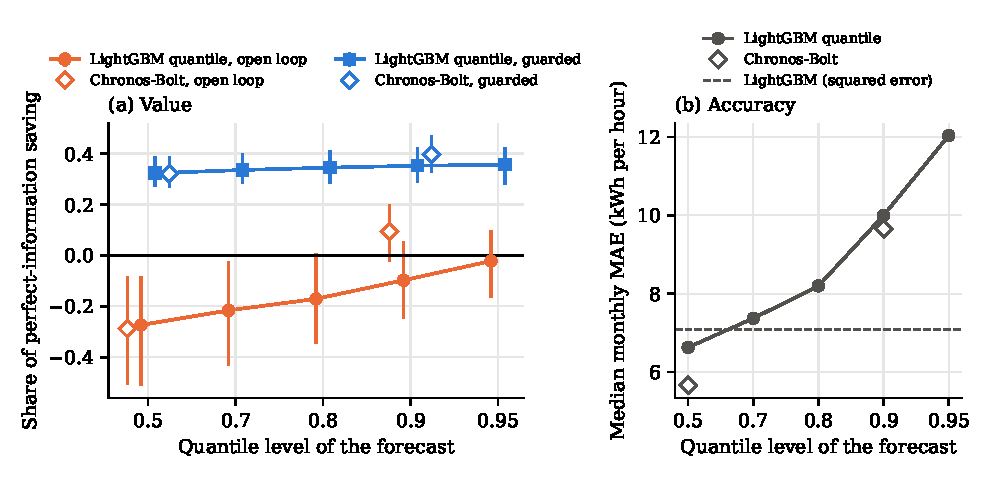
\includegraphics[width=\linewidth]{figures/fig_quantile_value.pdf}
\caption{Value and accuracy against the quantile level of the forecast (exploratory, added after the pre-specified study; demand-charge tariff, base battery). (a) Annual share of the perfect-information saving, medians and interquartile ranges over \res{nKept} buildings, for LightGBM quantile models (filled markers) and for the median and 0.9 quantile of the zero-shot Chronos-Bolt model (open diamonds), open loop and guarded. (b) Median monthly MAE; the dashed line is LightGBM trained on the squared error (F4).}\label{fig:quant}
\end{figure}

\subsection{A headroom margin in the day-ahead program}\label{sec:explore-headroom}
The open-loop failures arise because the program~\eqref{eq:lp} charges until the forecast grid draw touches the month-to-date peak (Section~\ref{sec:results}). The simplest robust remedy is a margin: we added the constraint $g_t+m\hat L_t\le z$, which keeps the planned grid draw at least a fraction $m$ of the forecast load below the planned peak, with $m=5\%$ and $10\%$. The margin changes the answer to H1 (Table~\ref{tab:headroom}). With $m=10\%$ the mean Kendall $\tau$ between MAE and value was $\res{rvHtenOpen}$ (CI $\res{rvHtenOpenLo}$ to $\res{rvHtenOpenHi}$) open loop and $\res{rvHtenGuard}$ with the guard. The null result of H1 is therefore specific to the plain program; with a robust margin, accuracy carries some information about value. The asymmetric score remained more informative ($\tau=\res{rvHtenPin}$ for the 0.9 pinball loss), F5 remained the most valuable of the five forecasters under both controllers, and the margin reduced but did not remove the open-loop damage: the four unbiased forecasters still raised the bill in \res{rvHtenUpFourLo}--\res{rvHtenUpFourHi}\% of buildings, against \res{rvHtenFfiveUp}\% for F5, the only one of the five with a positive median open-loop share ($\res{rvHtenFfiveSh}$). The guard remained the larger lever; combined with the 10\% margin it raised the median guarded saving to \res{rvHtenGPctLo}--\res{rvHtenGPctHi}\% of the bill.

\subsection{Accuracy at a fixed bias}\label{sec:explore-fe}
If accuracy were irrelevant, a lower MAE would not help even among forecasters with the same bias. A within-building regression of the annual share of F1--F5 on their relative MAE and relative bias, with building fixed effects and standard errors clustered by building (\res{rvFeN} building-forecaster observations), separates the two. Open loop, a percentage point of relative MAE changed the share by $\res{rvFeMaeOpen}$ (standard error \res{rvFeMaeSeOpen}) and a percentage point of over-forecast bias by $\res{rvFeBiasOpen}$ (\res{rvFeBiasSeOpen}); with the guard the MAE coefficient was similar, $\res{rvFeMaeGuard}$ (\res{rvFeMaeSeGuard}), and the bias coefficient almost vanished, $\res{rvFeBiasGuard}$ (\res{rvFeBiasSeGuard}). Accuracy therefore matters once the sign of the error is held fixed. The MAE fails as a ranking because the most valuable forecaster is the biased one, and the guard removes most of the reward for bias.

\subsection{A monthly hindsight benchmark}\label{sec:explore-hind}
The perfect-information benchmark is the daily program run on the actual load, which cannot plan the battery across the days of a month. A linear program over each whole calendar month with the actual load, the monthly hindsight optimum, bounds it. Under T1 the hindsight optimum saved a median \res{rvHindPct}\% of the annual bill against \res{rvHindDailyPct}\% for the daily benchmark, so that the daily benchmark captured a median \res{rvHindCapt}\% of the hindsight saving (interquartile range \res{rvHindCaptLo}--\res{rvHindCaptHi}\%); under T2 it captured \res{rvHindCaptTtwo}\%. Measured against the hindsight optimum instead of the daily benchmark, the median annual shares of the five forecasters, open loop and guarded, and of the reactive rule changed by at most \res{rvHindMaxDiff} (guarded F5, for example: \res{rvHindShGF5}). The myopia of the benchmark is therefore small here and does not explain the results.

\section{Discussion}\label{sec:discussion}

\paragraph{Implications for practice} Three recommendations follow for operators of behind-the-meter storage under demand charges. First, choose and tune a forecaster with an asymmetric score that penalises under-forecasts more than over-forecasts, such as the pinball loss of an upper quantile, not with the MAE. An upper-quantile point forecast is the optimal forecast under such a loss~\cite{gneiting2011point}, it needs no special training method, and here it was the most valuable forecaster although it was the least accurate. Second, never execute a cost-minimising day-ahead schedule open loop: the schedule charges up to the month's peak by design, and any under-forecast at those hours sets a new peak. A guard that refuses to charge into the peak and discharges against it turned every forecaster from a loss into a saving and mattered more than the choice of forecaster. Third, check the bill, not the error, on the operator's own buildings before deploying a forecaster; the attainable saving is a fraction of a per cent of the bill, so small systematic errors decide its sign. Under a pure time-of-use tariff, by contrast, a seasonal naive forecast was as good as any.

\paragraph{Implications for research} The results support the motivation of decision-focused learning~\cite{donti2017task,elmachtoub2022spo,mandi2024dfl} and qualify it. MAE is a poor proxy for value in this decision, but most of the gap is closed by a fixed asymmetric score, without training on the decision. Studies of decision-focused forecasters for storage~\cite{kim2025neural,depoortere2026dfl} should therefore include two baselines: a quantile forecaster, since part of their gain may come from the bias that training on decision cost induces; and a guarded controller, since a gain measured with open-loop execution may disappear once the controller corrects the schedule in real time. Benchmarks of building load forecasting~\cite{emami2023buildingsbench,miller2020gepiii} could report an asymmetric or decision-based score alongside their error metrics, as control benchmarks already score controllers by cost~\cite{vazquez2019citylearn}.

\paragraph{Limitations} The study uses one data set, with buildings from \res{keptSites} sites in 2016--2017, most of them on university campuses, and hourly data, so demand is billed on the hourly rather than the 15-minute peak. The tariff and the battery are stylised and the same for every building, and battery degradation and capital cost are ignored; the savings in dollars indicate magnitudes only. The schedule is a daily linear program that sees the month-to-date peak but not the rest of the month, and the two controllers are simple; a model predictive controller that re-optimises during the day~\cite{mary2025rmpc} would likely narrow the gap between forecasters further. Temperature is observed rather than forecast, the models are not refitted during the test year, and the synthetic errors are deliberately simple. The analysis plan was fixed in the author's own repository rather than with an independent registry, and three amendments were made, the last after the results and a review were seen; the registered test gave the same answer on the registered and the corrected simulation, and the conclusions about the sign of the error rest on secondary and exploratory analyses that a confirmatory study should test on new buildings.

\section{Conclusion}\label{sec:conclusion}

We asked whether a more accurate load forecast lowers a building's bill when it is used to schedule a battery, and answered with a pre-registered study of \res{nKept} buildings. Under a demand charge it did not: accuracy metrics did not rank five standard forecasters by their saving, the peak-conservative forecaster, least accurate on average, saved the most, and at equal error the direction and timing of the error mattered far more than its size. How the schedule was executed mattered more still, since open-loop schedules raised the bill in most buildings while a simple real-time guard made every forecaster profitable. Without a demand charge, accuracy did not matter at all. Forecasts for storage should be evaluated by the decisions they lead to, under the controller that will use them.

\section*{CRediT authorship contribution statement}
\textbf{Thanh Van Nguyen:} Conceptualization, Methodology, Software, Formal analysis, Data curation, Writing -- original draft, Writing -- review \& editing.

\section*{Declaration of generative AI and AI-assisted technologies in the writing process}
During the preparation of this work the author used Claude (Anthropic) to write and test the analysis code, to search for literature and check every reference against Crossref and arXiv, and to draft and edit the text. The research question, the pre-registered design and the interpretation of the results were reviewed by the author. After using this tool, the author reviewed and edited the content as needed and takes full responsibility for the content of the published article.

\section*{Declaration of competing interest}
The author declares no known competing financial interests or personal relationships that could have appeared to influence the work reported in this paper.

\section*{Data availability}
The Building Data Genome 2 data are public under the CC BY-SA 4.0 licence~\cite{miller2020bdg2}. The analysis plan with its amendments, the code, the download script with file hashes, the result files and the outputs of the six-building pipeline check are available at \url{\repoURL}.

\section*{Funding}
This research did not receive any specific grant from funding agencies in the public, commercial, or not-for-profit sectors.


\bibliographystyle{elsarticle-num}
\bibliography{refs}

\end{document}
